\documentclass{article}
\usepackage[utf8x]{inputenc}
\usepackage[frenchb]{babel}
\usepackage[T1]{fontenc}
\usepackage{lmodern}
\usepackage{fullpage}
\usepackage{graphicx}
\usepackage{epstopdf}
\usepackage{caption}
\usepackage{subcaption}
\usepackage{multirow}
\usepackage{placeins}
% Math symbols
\usepackage{amsmath}
\usepackage{amssymb}
\usepackage{amsthm}
% Numbers and units
\usepackage[squaren, Gray]{SIunits}
\usepackage{sistyle}
%\usepackage[autolanguage]{numprint}
%\usepackage{numprint}
\newcommand\si[2]{\numprint[#2]{#1}}
\newcommand\np[1]{\numprint{#1}}


\DeclareMathOperator{\pgcd}{pgcd} % use \dif instead

\DeclareMathOperator{\newdiff}{d} % use \dif instead
\newcommand{\dif}{\newdiff\!}
\newcommand{\fpart}[2]{\frac{\partial #1}{\partial #2}}
\newcommand{\ffpart}[2]{\frac{\partial^2 #1}{\partial #2^2}}
\newcommand{\fdpart}[3]{\frac{\partial^2 #1}{\partial #2\partial #3}}
\newcommand{\fdif}[2]{\frac{\dif #1}{\dif #2}}
\newcommand{\ffdif}[2]{\frac{\dif^2 #1}{\dif #2^2}}
\newcommand{\constant}{\ensuremath{\mathrm{cst}}}
\newcommand{\bigoh}{\ensuremath{\mathcal{O}}}

% cfr http://en.wikibooks.org/wiki/LaTeX/Colors
\usepackage{color}
\usepackage[usenames,dvipsnames,svgnames,table]{xcolor}
\definecolor{dkgreen}{rgb}{0.25,0.7,0.35}
\definecolor{dkred}{rgb}{0.7,0,0}

\usepackage{listings}
\lstset{
  numbers=left,
  numberstyle=\tiny\color{gray},
  basicstyle=\rm\small\ttfamily,
  keywordstyle=\bfseries\color{dkred},
  frame=single,
  commentstyle=\color{gray}=small,
  stringstyle=\color{dkgreen},
  %backgroundcolor=\color{gray!10},
  %tabsize=2,
  rulecolor=\color{black!30},
  %title=\lstname,
  breaklines=true,
  framextopmargin=2pt,
  framexbottommargin=2pt,
  extendedchars=true,
  inputencoding=utf8x
}
\lstset{language={matlab}}

\title{Optimisation devoir 2 \\
Synthèse robuste d'antennes}
\author{Quentin Laurent \and Nicolas Stevens}

\newcommand{\I}{\mathcal{I}}
\newcommand{\lmax}{\lambda_\mathrm{max}}
\newcommand{\lmin}{\lambda_\mathrm{min}}

\usepackage{listings}
\usepackage{color}
\usepackage{textcomp}
\definecolor{listinggray}{gray}{0.9}
\definecolor{lbcolor}{rgb}{0.9,0.9,0.9}

%Pour insertion de codes matlab...
\lstset{
	backgroundcolor=\color{lbcolor},
numbers=left,
%
	tabsize=4,
	rulecolor=,
	language=matlab,
        basicstyle=\scriptsize,
        upquote=true,
        aboveskip={1.5\baselineskip},
        columns=fixed,
        showstringspaces=false,
        extendedchars=true,
        breaklines=true,
        prebreak = \raisebox{0ex}[0ex][0ex]{\ensuremath{\hookleftarrow}},
        frame=single,
        showtabs=false,
        showspaces=false,
        showstringspaces=false,
        identifierstyle=\ttfamily,
        keywordstyle=\color[rgb]{0,0,1},
        commentstyle=\color[rgb]{0.133,0.545,0.133},
        stringstyle=\color[rgb]{0.627,0.126,0.941},
}
\begin{document}
\maketitle
\section*{Introduction}
Soit une poutre de section carré et de longueur "infinie" soumise à une charge $F$ sur sa moitié centrale supérieur. On se propose d'étudier la résistance de cette poutre lorsqu'elle est chargée verticalement. On définie le champs de contraintes $\sigma = \begin{pmatrix}
\sigma_{xx} & \sigma_{xy}\\
\sigma_{xy} & \sigma_{yy}
\end{pmatrix}$. On souhaite maximiser la charge imposée (c'est à dire l'intégrale de $\sigma_{yy}$ sur la surface supérieur de la poutre) sans qu'il y ait déformation plastique, sous les contraintes mécaniques suivantes : 
\begin{align}
\frac{\partial \sigma_{xx}}{\partial x} + \frac{\partial \sigma_{xy}}{\partial y} &= 0 \label{eq:contrainteequilibre1}\\
\frac{\partial \sigma_{xy}}{\partial x} + \frac{\partial \sigma_{yy}}{\partial y} &= 0\label{eq:contrainteequilibre2}\\
\sigma^{(i)}n &= \sigma^{(j)}n & \text{si le triangles $(i)$ et $(j)$ ont un côté de normale $n$ en commun} \label{eq:contrainteContinuite}\\
\sigma n &= 0 & \text{sur les frontières latérales} \label{eq:contrainteFrontiere} \\
(\sigma_{xx} - \sigma_{yy})^2 + (2 \sigma_{xy})^2 & \leq 4 k^2 \label{eq:contrainteTresca}\\
\end{align}
où les contraintes \eqref{eq:contrainteequilibre1} et \eqref{eq:contrainteequilibre2} expriment la conservation de la quantité de mouvement; et la contrainte \eqref{eq:contrainteTresca} est le critère de plasticité de Tresca-von Mises. 


Comme ce problème possède une infinité de contraintes (problème continu), nous le discrétisons en triangles comme à la figure \ref{fig:discretisation}. Un nœud peut prendre plusieurs valeurs $\sigma$ si il appartient à plusieurs triangles. 

\begin{figure}[h!]
\centering
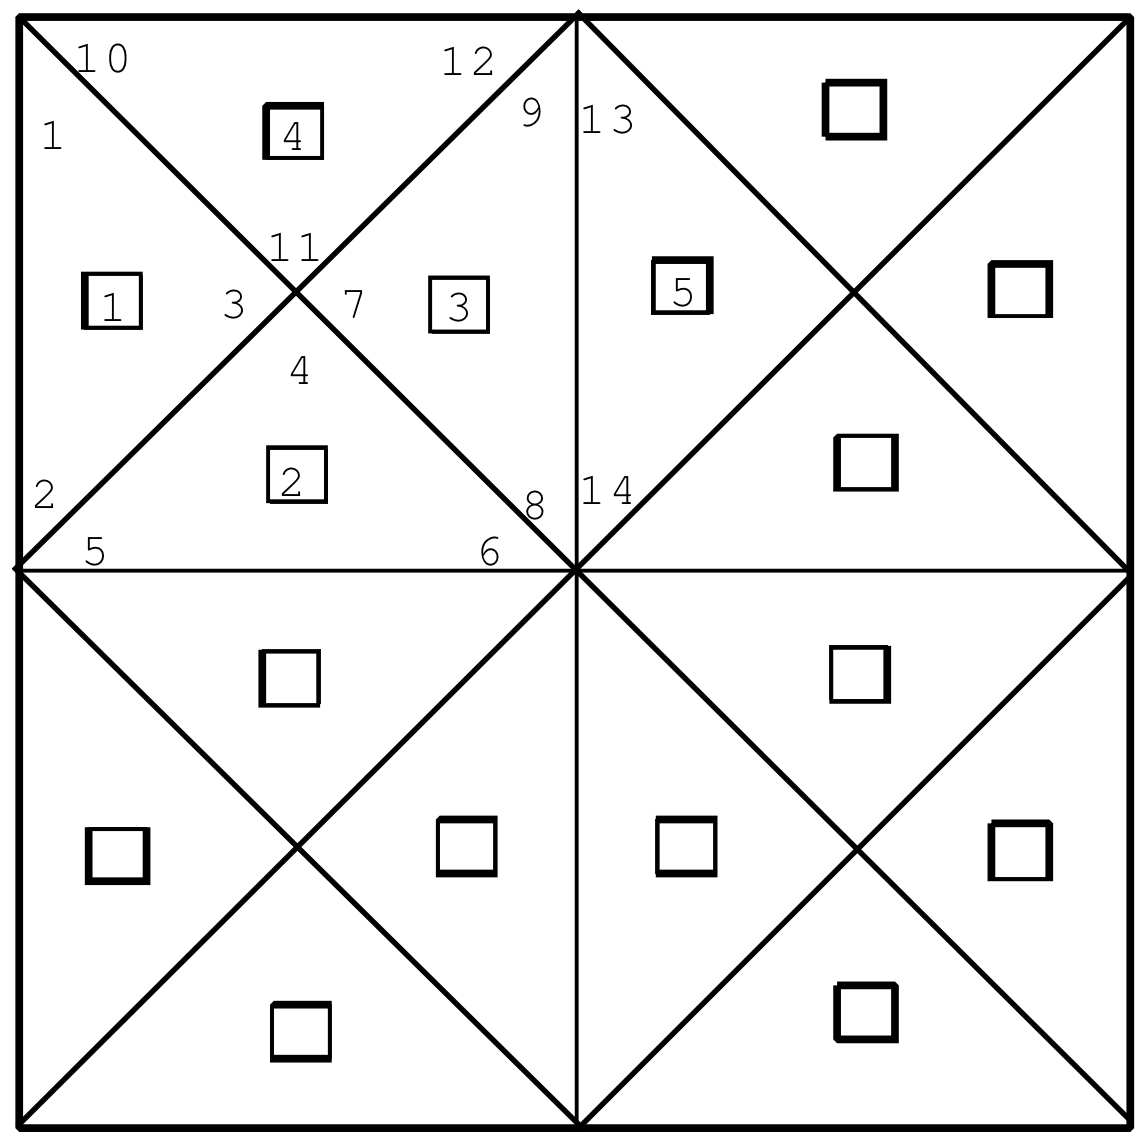
\includegraphics[height=5cm]{images/discretisation.png}
\caption{Section de la poutre discrétisée en triangles}
\label{fig:discretisation}
\end{figure}


\newpage
\section{Modélisation}
On souhaite formuler les contraintes mécaniques précédentes dans le cas discrétisé, comme des contraintes d'un problème convexe.\\

Soit $L$ la longueur d'un côté de la poutre. On défini $l=\frac{L}{N}$, la longueur d'un côté d'un carré et $h=\frac{l}{2}$, la longueur de la hauteur d'un triangle (un demi carré). On considère quatre cas de triangles : 
\begin{itemize}
\item cas triangle 1, orienté comme le 1 sur la figure \ref{fig:discretisation};
\item cas triangle 2, orienté comme le 2 sur la figure \ref{fig:discretisation};
\item cas triangle 3, orienté comme le 3 sur la figure \ref{fig:discretisation};
\item cas triangle 4, orienté comme le 4 sur la figure \ref{fig:discretisation};
\end{itemize} 
et dans chacun des cas, on écrit les conditions de divergence nulle comme des différences finies. 

Pour les conditions de continuité, on distingue également quatre cas : 
\begin{equation}
\overrightarrow{n} = \begin{pmatrix}
1\\
-1
\end{pmatrix}, 
\overrightarrow{n} = \begin{pmatrix}
1\\
1
\end{pmatrix}, 
\overrightarrow{n} = \begin{pmatrix}
1\\
0
\end{pmatrix},
\overrightarrow{n} = \begin{pmatrix}
0\\
1
\end{pmatrix}
\end{equation}

La fonction objectif correspond à une règle des trapèze sur les $\sigma_{yy}$ des triangles en lesquels le bloc exerce la force (appelons cet ensemble $\mathcal{F}$. Il s'agit de triangles de type 4. Nous appelons les sommets supérieurs de chacun des ces triangles 1 et 3). Cela donne
\begin{align*}
\max \sum_{i \in \mathcal{F}} L \frac{\sigma_{yy}^1 + \sigma_{yy}^3}{2}
\end{align*}

Les conditions de continuité donnent, en nommant $a,b$ les points d'un coté du segment et $c,d$ les points de l'autre coté : \\
\begin{center}
\begin{minipage}{0.4\textwidth}
\textbf{cas 1 : }
\begin{align*}
\sigma_{xx}^a - \sigma_{xy}^a &= \sigma_{xx}^c - \sigma_{xy}^c \\
 \sigma_{xy}^a - \sigma_{yy}^a &= \sigma_{xy}^c - \sigma_{yy}^c \\
 \sigma_{xx}^b - \sigma_{xy}^b &= \sigma_{xx}^d - \sigma_{xy}^d \\
 \sigma_{xy}^b - \sigma_{yy}^b &= \sigma_{xy}^d - \sigma_{yy}^d \\
\end{align*}
\end{minipage}
\vline
\begin{minipage}{0.4\textwidth}
\textbf{cas 2 :}
\begin{align*}
\sigma_{xx}^a + \sigma_{xy}^a &= \sigma_{xx}^c + \sigma_{xy}^c \\
 \sigma_{xy}^a + \sigma_{yy}^a &= \sigma_{xy}^c + \sigma_{yy}^c \\
 \sigma_{xx}^b +\sigma_{xy}^b &= \sigma_{xx}^d + \sigma_{xy}^d \\
 \sigma_{xy}^b + \sigma_{yy}^b &= \sigma_{xy}^d + \sigma_{yy}^d \\
\end{align*}
\end{minipage}

\begin{minipage}{0.4\textwidth}
\textbf{cas 3 :}
\begin{align*}
\sigma_{xx}^a &= \sigma_{xx}^c \\
 \sigma_{xy}^a  &= \sigma_{xy}^c \\
 \sigma_{xx}^b&= \sigma_{xx}^d\\
 \sigma_{xy}^b &= \sigma_{xy}^d  \\
\end{align*}
\end{minipage}
\vline
\begin{minipage}{0.4\textwidth}
\textbf{cas 4 :}
\begin{align*}
\sigma_{xy}^a &= \sigma_{xy}^c \\
\sigma_{yy}^a &=  \sigma_{yy}^c \\
\sigma_{xy}^b &= \sigma_{xy}^d \\
\sigma_{yy}^b &= \sigma_{yy}^d \\
\end{align*}
\end{minipage}
\end{center}

Les conditions d'équilibre donnent : 
\begin{align*}
\frac{\sigma_{xx}^3 - \frac{\sigma_{xx}^1+\sigma_{xx}^2}{2}}{h} + \frac{\sigma_{xy}^1-\sigma_{xy}^2}{l}&=0 & \text{pour triangle type 1}\\
\frac{\sigma_{xy}^3 - \frac{\sigma_{xy}^1+\sigma_{xy}^2}{2}}{h} + \frac{\sigma_{yy}^1-\sigma_{yy}^2}{l}&=0& \text{pour triangle type 1}\\
\frac{\sigma_{xx}^3-\sigma_{xx}^2}{l} + \frac{\sigma_{xy}^1 - \frac{\sigma_{xy}^3+\sigma_{xy}^2}{2}}{h} &=0& \text{pour triangle type 2}\\
\frac{\sigma_{xy}^3-\sigma_{xy}^2}{l} + \frac{\sigma_{yy}^1 - \frac{\sigma_{yy}^3+\sigma_{yy}^2}{2}}{h} &=0 & \text{pour triangle type 2}\\
\frac{\frac{\sigma_{xx}^3+\sigma_{xx}^2}{2} - \sigma_{xx}^1 }{h} + \frac{\sigma_{xy}^3-\sigma_{xy}^2}{l}&=0& \text{pour triangle type 3}\\
\frac{\frac{\sigma_{xy}^3+\sigma_{xy}^2}{2} - \sigma_{xy}^1 }{h} + \frac{\sigma_{yy}^3-\sigma_{yy}^2}{l}&=0& \text{pour triangle type 3}\\
\frac{\sigma_{xx}^3-\sigma_{xx}^1}{l} + \frac{\frac{\sigma_{xy}^1+\sigma_{xy}^3}{2} - \sigma_{xy}^2 }{h} &=0 & \text{pour triangle type 4}\\
\frac{\sigma_{xy}^3-\sigma_{xy}^1}{l} + \frac{\frac{\sigma_{yy}^1+\sigma_{yy}^3}{2} - \sigma_{yy}^2 }{h} &=0 & \text{pour triangle type 4}\\
\end{align*}


Les conditions frontières latérales donnent, pour tout nœud $a$ appartenant à une frontière latérale : 
\begin{align*}
\sigma_{xx}^a&= 0\\
 \sigma_{xy}^a &= 0  \\
\end{align*}

Les conditions frontières supérieurs donnent, pour tout nœud $a$ appartenant au premier quart ou au dernier quart de la frontière supérieur (en fait c'est un peu plus subtil que ça, comme $N$ n'est pas toujours un multiple de 4, on a $2\lfloor \frac{N}{4} \rfloor + 1 \left( \lceil \frac{N}{4} \rceil - \lfloor \frac{N}{4} \rfloor \right) = \lfloor \frac{N}{4} \rfloor + \lceil \frac{N}{4} \rceil$ points en lesquels il faut imposer une contrainte de chaque côté du bloc exerçant la force; c'est-à-dire au total $4*\left(  \lfloor \frac{N}{4} \rfloor + \lceil \frac{N}{4} \rceil \right)$ contraintes) : 
\begin{align*}
\sigma_{yy}^a&= 0\\
 \sigma_{xy}^a &= 0  \\
\end{align*}


Toutes les contraintes énoncée précédemment forment un système $Ax=b$. A cela viennent s'ajouter les contraintes de von Mises qui sont convexes. Notre problème d'optimisation est donc convexe et s'écrit 
\begin{align*}
& \max c^T x\\
 Ax &= b\\
 x & \in \mathcal{X}
\end{align*}
où $\mathcal{X}$ est l'ensemble décrit par les contraintes de von Mises. L'appartenance à cet ensemble sera imposer au moyens de fonctions barrières (voir méthodes des point intérieur). 

Si on fait un bilan. Soit $N$ le nombre de carrés sur un côté de la section de la poutre, alors on a : $\text{\# carrés  } = N^2$, $\text{\# triangles  } = 4N^2$, $\text{\# points  } = 12 N^2$, $\text{\# contraintes  } = 24N^2+12N(N-1)+8N + 4*\left(  \lfloor \frac{N}{4} \rfloor + \lceil \frac{N}{4} \rceil \right)$.
Pour $N=4$ par exemple, on a $520$ contraintes.

\paragraph{Solution optimale du problème discret : } L'idée de base des éléments finis est d'approcher l'ensemble des solutions $\mathcal{U}$ par un ensemble approché $\mathcal{U}_h$. Typiquement, un ensemble de polynômes d'interpolations. Cet ensemble respecte bien sûr $\mathcal{U}_h \subset \mathcal{U}$. La dimension de cet ensemble croit avec les degrés de libertés par élément (degré du polynôme d'interpolation sur chaque élément); et croit aussi avec le nombre d'éléments. Dans notre cas, on a choisi d'interpoler linéairement la solution sur chaque triangle. La dimension de l'espace des solutions discrètes $\mathcal{U}_h$ croit donc juste avec le nombre de triangles. 

Il est donc important de se rendre compte qu'en résolvant le problème discret, on résout une \textbf{restriction} du problème initial et par conséquent, l'objectif est moins élevé que le véritable objectif (donc la charge optimale discrète est moins élevé que la charge optimale réelle; ce qui n'est pas un problème vu qu'on souhaite calculer une charge limite avant rupture, donc on préfère trouver une charge limite plu petite que plus grande). Vraisemblablement au plus on aura de triangles, au plus on aura un espace de solutions grand, et au plus l'objectif (la charge limite optimale) sera élevé.


\section{Méthode de point intérieur}

Nous cherchons à définir une méthode à pas longs pour un problème d'optimisation du type suivant :
\begin{align*}
\min_{x_1,x_2} & c_1^Tx_1+c_2^Tx_2\\
\begin{pmatrix} A_1 & A_2 \end{pmatrix}
& = \begin{pmatrix} x_1 \\ x_2 \end{pmatrix} \\
x_1 & \geq 0 \\
x_2 & \in \mathbb{L}^{n_2}
\end{align*}
A cet effet nous supprimons les contraintes d'inégalité à l'aide de fonctions barrières. Le problème perturbé s'écrit donc
\begin{align*}
\min_{x_1,x_2}  & c_1^Tx_1+c_2^Tx_2 - \mu_k(\sum_{x_1i} \log(x_i)+ \log(\tau^2 - ||x_2||_2^2)) \\
\begin{pmatrix} A_1 & A_2 \end{pmatrix}
& = \begin{pmatrix} x_1 \\ x_2 \end{pmatrix} \\
\end{align*}
Comme le problème est convexe, nous pouvons écrire les conditions d'optimalité comme suit :
\begin{align*}
\bigtriangledown f & =  0 \\
\text{avec }f(x_1,x_2,z) & = 
c_1^Tx_1+c_2^Tx_2 - \mu_k(\sum_{x_1i} \log(x_i)+ \log(\tau^2 - ||x_2||_2^2)) -z^T(A_1x_1+A_2x_2-b)\\
& \Rightarrow & \\
\bigtriangledown_{x_1}f & =  c_1^T -s_1^T -z^TA_1 = 0 \\
\bigtriangledown_{x_2}f & =  c_2^T -s_2^T - z^TA_2 = 0 \\
\bigtriangledown_{z}f & =  -x_1^TA_1^T-x_2^TA_2^T+b^T = 0 \\
s_{1i} x_{1i} & = \mu_k \\
s_{2i} \frac{\tau^2 - ||x_{2}||_2^2}{2x_{2i}} & = \mu_k
\end{align*}
Où $z$ est le vecteur des multiplicateurs de Lagrange. On doit donc résoudre $F=0 $ avec 
$$
F : \begin{pmatrix}
x_1 \\ x_2 \\ y \\ s_1 \\ s_2 \\ t
\end{pmatrix}
\rightarrow
\begin{pmatrix}
A_1x_1+A_2x_2-b \\
A^T_1y + s_1 -c_1 \\
A_2^Ty + s_2 - c_2 \\
X_1S_1e - \mu_k e \\
TS_2e - \mu_ke \\
2X_2Te - (\tau^2-||x_2||_2^2)e
\end{pmatrix}
$$
On peut calculer la jacobienne : 
$$J_F = \begin{pmatrix}
A_1 & A_2 & 0 & 0 & 0 & 0 \\
0 & 0 & A_1^T & I & 0 & 0 \\
0 & 0 & A_2^T & 0 & I & 0 \\
S_1 & 0 & 0 & X_1 & 0 & 0 \\
0 & 0 & 0 & 0 & T & S_2 \\
0 & 2T + 2ex_2^T & 0 & 0 & 0 & 2X_2 

\end{pmatrix}$$
On a alors le système à résoudre pour obtenir le pas de Newton

\begin{align}
J_F \begin{pmatrix}
\Delta x_1 \\
\Delta x_2 \\
\Delta y \\
\Delta s_1\\
\Delta s_2\\
\Delta t\\
\end{pmatrix} & = & \begin{pmatrix}
0 \\
0\\
0\\
-X_1S_1e+\mu_k e \\
-TS_2e + \mu_k e\\
-2X_2Te+ (\tau^2-||x_2||_2^2)e\\
\end{pmatrix}
\label{eq:pasN}
\end{align}
On a alors l'algorithme suivant
\begin{algorithm}[!h]
\KwData{$A_1,A_2,c_1,c_2,b,\tau_L,\mu_0, \epsilon,\sigma,\nu$}
$(x_1^{0},x_2^{0},y^{0},s_1^{0},s_2^{0},t^{0})$ est tel que 
$\delta(x_1^{0},x_2^{0},y^{0},s_1^{0},s_2^{0},t^{0}) < \nu$\;
\For{$k = 0,1,2,... $, }{
Calculer le pas de Newton $(\Delta x_1^{k},\Delta x_2^{k},\Delta y^{k},\Delta s_1^{k},\Delta s_2^{k},\Delta t^{k})$ à l'aide du système (\ref{eq:pasN})\;
Poser $x^{k+1} = x^k + \alpha_k \Delta x^k$}
%TODO : choix du alpha
\end{algorithm}
\section{Première formulation robuste}
\subsection{Modèle}

Afin de prendre en compte les erreurs sur les facteurs d'amplification $x_i$, nous utilisons les valeurs maximales des variations possibles de $\hat{D(\theta)}$ en chaque point de notre discrétisation. Nous imposons que malgré ces variations nous restons dans les intervalles voulus. On transforme par exemple la première contrainte $D(\theta)\leq \epsilon$ du modèle non robuste :
\begin{equation}
d(\theta)^T (x.*(1+\xi)) \leq \epsilon \Longleftrightarrow d(\theta)^T (x.*\xi) \leq \epsilon- d(\theta)^T x
\end{equation}
%Où $d(\theta)$ est le vecteur colonne contenant les $d_i(\theta)$ et $dx(\theta)$ le produit élément par élément de $d(\theta)$ avec $x$.
Nous cherchons à ce que notre optimum $(x,\epsilon)$ soit valable dans le pire cas, c'est-à-dire pour cette contrainte celui où $d(\theta)^T (x.*\xi)$ est maximum. Comme nous imposons également que $|\xi_i|\leq \tau$ nous formulons un problème de maximisation linéaire et imposons une condition sur son objectif: 
\begin{align*}
\max_{\xi_i} d(\theta)^T (x.*\xi)  & \leq  \epsilon- d(\theta)^T x \\
\xi_i & \leq \tau \\
-\xi_i & \leq \tau 
\end{align*}
Nous avons donc un problème d'optimisation dont l'optimum sera inférieur à $\epsilon- d(\theta)^T x $. On peut mettre ce problème sous forme duale. Par dualité forte on sait que l'objectif optimal de ce problème dual sera le même que celui du primal. Celà nous donnera :
\begin{align*}
\min_{y_+,y_-} \mathbf{1}^{n\times 1}\tau y_++\mathbf{1}^{n\times 1}\tau y_- & \leq \epsilon- d(\theta)^T x \\
y_+,y_-  & \geq  0 \\
(I,-I)\begin{pmatrix}
y_+ \\
y_-
\end{pmatrix}
& = 
\begin{pmatrix}
d_1(\theta)x_1 \\
d_2(\theta)x_2 \\
\vdots \\
d_n(\theta)x_n 
\end{pmatrix}
\end{align*}
Comme ce problème est un problème de minimisation, si la contrainte sur l'objectif est satisfaite pour n'importe quelle solution admissible, on sait que l'optimum satisfera aussi cette contrainte.\\
On peut alors revenir à notre problème de base dans lequel on remplace la contrainte $D(\theta)\leq \epsilon$ par les contraintes du dual et la contrainte sur l'objectif.
On traduit de la même manière les autres contraintes. On obtient alors le modèle suivant :

\begin{align*}
\min_{x,\epsilon ,y_1+,y_1-,y_2+,y_2-,y_3+,y_3-,y_4+,y_4-} \epsilon &  \\
y_{i+},y_{i-}  & \geq  0 \\
(I,-I)
 \begin{pmatrix}
y_i+ \\
y_i-
\end{pmatrix}
& = 
\begin{pmatrix}
d_1(\theta)x_1 \\
\vdots \\
d_n(\theta)x_n 
\end{pmatrix} \\
\forall i = 1,2,3,4\:\:
\forall \theta \in S_e \cup P_e  &  \\
\mathbf{1}^{n\times 1}\tau y_{1+}+\mathbf{1}^{n\times 1}\tau y_{1-} & \leq \epsilon -d(\theta)^Tx \\
\mathbf{1}^{n\times 1}\tau y_{2+}+\mathbf{1}^{n\times 1}\tau y_{2-} & \leq \epsilon + d(\theta)^Tx \\
\forall \theta \in S_e &  \\
\mathbf{1}^{n\times 1}\tau y_{3+}+\mathbf{1}^{n\times 1}\tau y_{3-} & \leq  \epsilon +1 -d(\theta)^Tx \\
\mathbf{1}^{n\times 1}\tau y_{4+}+\mathbf{1}^{n\times 1}\tau y_{4-} & \leq  \epsilon -1 + d(\theta)^Tx \\
\forall \theta \in P_e & 
\end{align*}
Cette formulation introduit $8N$ variables supplémentaires par rapport au modèle de base
%TODO : Pourquoi le solver utilise des itérations barrier et pas des simplexes?
\FloatBarrier
\subsection{Analyse des résultats}
Les figures \ref{fig:ModROBUST1} montrent les résultats obtenus pour différentes valeurs de $\tau$. Un récapitulatif des résultats pour les différents modèle est donné à la table \ref{table:Recap}.\\
\begin{itemize}
\item Dans le cas $\tau = 0.001$, on constate une augmentation du $\epsilon$ par rapport au modèle de base. Les erreurs pour les $x_i$ perturbés sont cependant bien moindre. On constate également que les erreurs pour des $x_i$ perturbés avec une perturbation de l'ordre de $\tau=0.001$ ou de $\tau = 0.01$ sont moindre que dans le modèle avec $\tau=0.01$. Cependant, on observe des dépassements pour certaines réalisation des $\xi_i$ si on applique les perturbations de $\tau=0.01$. (ce qui est logique vu que le modèle n'est pas conçu pour résister à de telles perturbations). On constate que l'ordre de grandeur des $x_i$ non-nuls est inférieur à celui du modèle de base ce qui confirme notre intuition comme quoi le modèle robuste a tendance à fournir des $x_i$ plus petits.\\ 
 \item Dans le cas $\tau = 0.01$, on constate toujours une augmentation du $\epsilon$ par rapport au modèle de base et au modèle où $\tau = 0.001$. Les erreurs pour les $x_i$ perturbés sont plus grande que dans le modèle $\tau=0.001$ pour des perturbations de l'ordre de $\tau = 0.001$ et $\tau=0.01$, mais le modèle ne présente jamais de dépassement. On constate que l'ordre de grandeur des $x_i$ non-nuls est inférieur à celui du modèle $\tau=0.001$, ce qui confirme encore notre intuition.
\end{itemize}

\begin{figure}[h!]
  \centering
  \begin{subfigure}[b]{0.32\textwidth}
  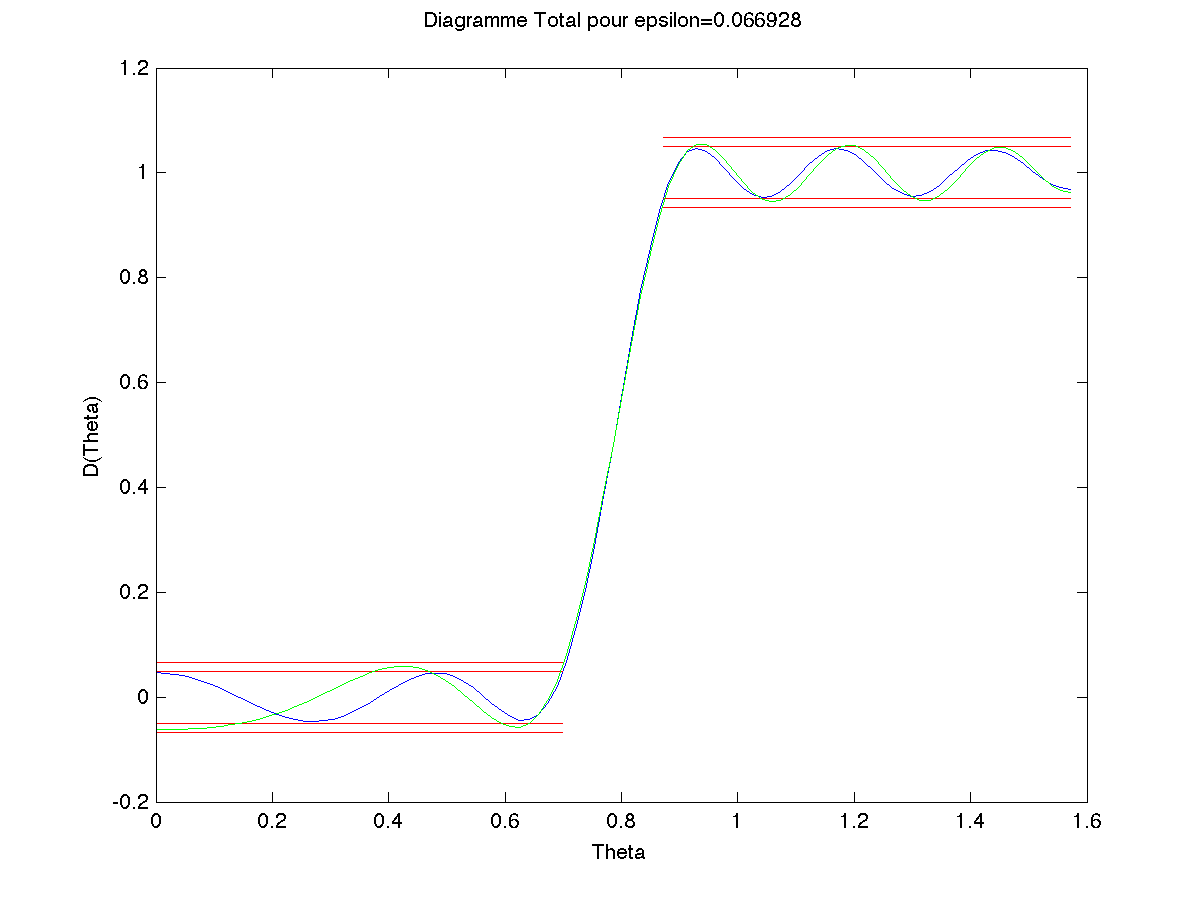
\includegraphics[width=\textwidth]{D-ModRobust1.png}
  \caption{$D(\theta)$ pour le modèle $\tau = 0.01$ (en vert) et $\tau = 0.001$ (en bleu) et $x$ non-perturbé.}
  \label{fig:D-ModRobust1}
  \end{subfigure}
  ~ 
 \begin{subfigure}[b]{0.32\textwidth}
  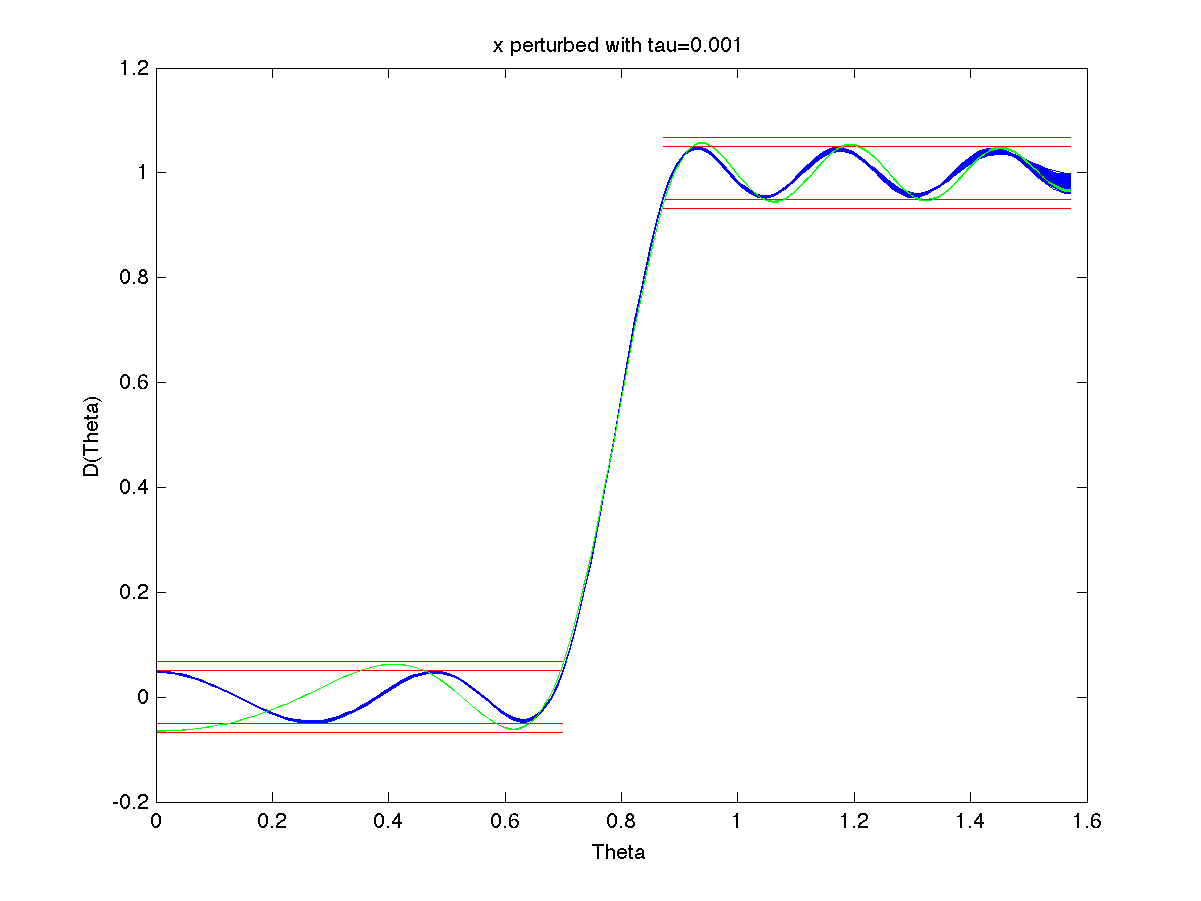
\includegraphics[width=\textwidth]{D-ModRobust1-test3Rob001.png}
  \caption{$D(\theta)$ pour une perturbation de $\tau = 0.001$ sur les $x$ (en vert pour un modèle de $\tau=0.01$ en bleu pour $\tau=0.001$).}
  \label{fig:D-ModRobust1-test3RobTau001}
  \end{subfigure}
  ~ 
  \begin{subfigure}[b]{0.32\textwidth}
  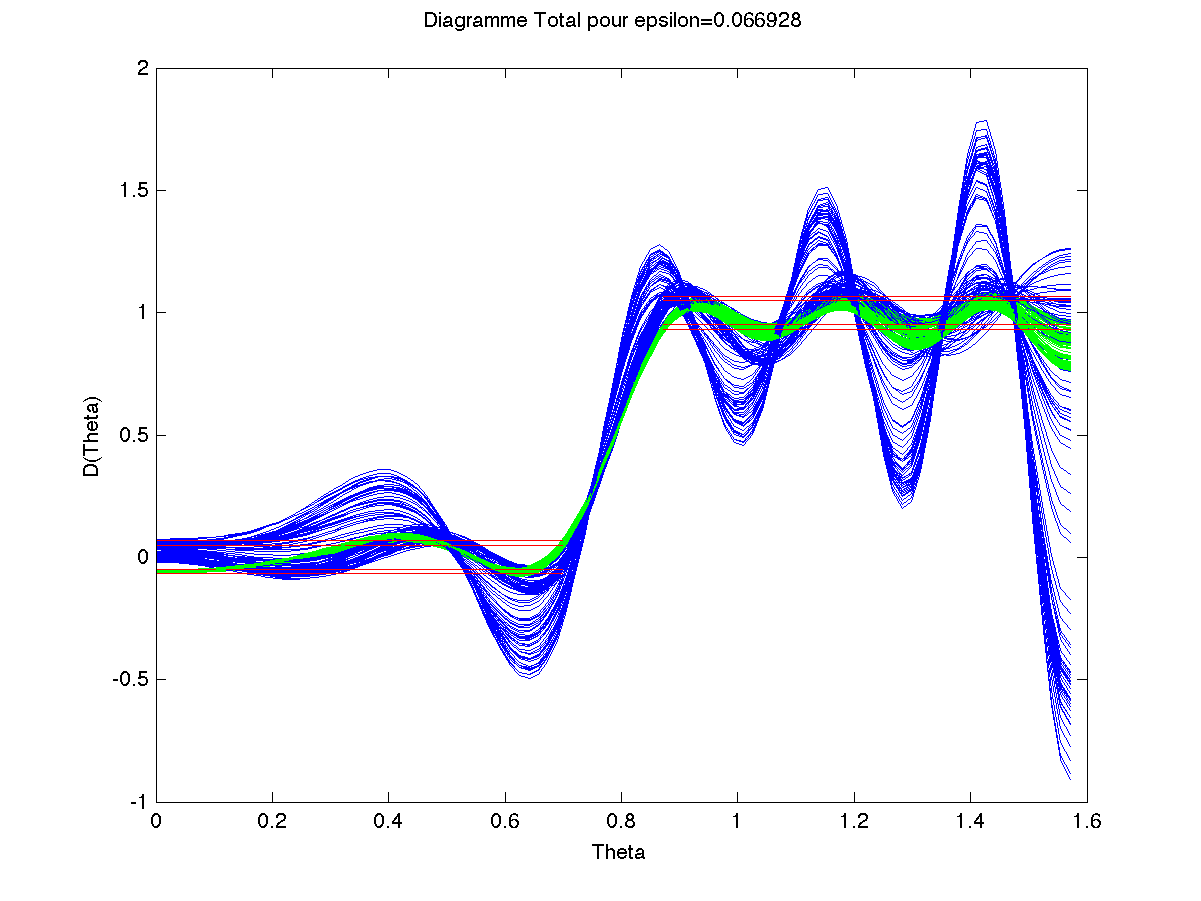
\includegraphics[width=\textwidth]{D-ModRobust1-test3Rob01.png}
  \caption{$D(\theta)$ pour une perturbation de $\tau = 0.01$ sur les $x$ (en vert pour un modèle de $\tau=0.01$ en bleu pour $\tau=0.001$).}
  \label{fig:D-ModRobust1-test3RobTau01}
  \end{subfigure}
\caption{Les deux derniers graphes sont donnés pour une centaine de réalisations des $\xi_i$.}
\label{fig:ModROBUST1}
  \end{figure}

\begin{table}
\centering
\begin{tabular}{c|c|c|ccc}
 & & &  &\textbf{Erreurs pour : } &\\
 & $\epsilon$ & $\mathcal{O}( x_i)$ ($x_i\neq0$ &$x_i$ & $x_i$ pert. ($\tau=0.001$) & $x_i$ pert. ($\tau=0.01$) \\
 \hline
Modèle de base & $2\%$ & $10^3$ &0.0185 & 5.3977 & 47.9054 \\
Modèle robuste 1 ($\tau=0.001$) & $5.07 \%$ & $10^0$& 0.0396 & 0.0396  & 0.0440 \\
Modèle robuste 1 ($\tau=0.01$)  & $6.80 \%$ &$10^{-1}$ &0.0508 & 0.0508 & 0.0510 \\
\end{tabular}
\caption{Récapitulatif des résultats des erreurs et de la borne maximal $\epsilon$ obtenus pour les différents modèles et les différents types de perturbations.}
\label{table:Recap}
\end{table}
\FloatBarrier
\section{Seconde formulation robuste}
\subsection{Modèle}
Le modèle robuste linéaire se base sur le pire des cas possible pour calculer un $epsilon$ optimal. On impose maintenant que
$$\sum_{i=1}^N \xi_i^2 \leq \gamma^2$$
On veut choisir une valeur de $\gamma$ telle que $P(\sum_{i=1}^N \xi_i^2 \leq \gamma^2)\geq 0.9999$. On va utiliser ici des variables intermédiaires $\xi_i^2$. La moyenne et la variance de ces variables sont $\mu = \frac{\tau^2}{3}$ et $\sigma^2 = \tau^4\cdot(\frac{1}{5}-\frac{1}{9})$.
Par le théorême central limite, on sait que la distribution $Z = \sum_{i=1}^N \xi_i^2$ tend vers une variable normale : $Z\sim \mathcal{N}(N\mu, N\sigma^2)$. Il suffi alors d'inverser la CDF de Z pour trouver $\gamma$ tel que $P(Z\leq \gamma^2)=0.9999$( v. table \ref{gamma} pour les résultats).
\begin{table}
\centering
\begin{tabular}{|c|c|c|}
\hline
$\tau$ & 0.001 & 0.01 \\
\hline
$\gamma$ & 0.0045107 & 0.045107 \\
\hline
\end{tabular}
\caption{Résultat de nos calculs pour $\gamma$}
\label{gamma}
\end{table}
%TODO : vérifier
On s'attend donc à de meilleurs résultats car les zones de $\mathbb{R}_N$ où tous les $\xi_i$ ont une valeur absolue élevée sont supprimées.
On peut à nouveau reprendre les contraintes du primal et reformuler un problème d'optimisation, conique cette fois. On écrit à nouveau une paire primal dual :
\begin{center}
\begin{minipage}{0.4\textwidth}
\begin{eqnarray}
\max_{\xi} dx^T \xi & \leq & \epsilon - d(\theta)^Tx \nonumber \\
\begin{pmatrix}t \\ \xi \end{pmatrix} & \in  & \mathbb{L}_{R^{n+1}} \nonumber \\ 
t = \gamma \nonumber
\end{eqnarray}
\end{minipage}
\begin{minipage}{0.4\textwidth}
\begin{eqnarray*}
\min_{y} \gamma^2 y & \leq & \epsilon - d(\theta)^Tx \\
\begin{pmatrix}
y \\
d_1(\theta)x_1(\theta) \\
\vdots \\
d_n(\theta)x_n(\theta)
\end{pmatrix}
 & \in & \mathbb{L}_{R^{n+1}}
\end{eqnarray*}
\end{minipage}
\end{center}
Par la dualité forte, l'objectif optimal du dual conique est supérieur à l'optimum du primal. Celà nous permet encore une fois de réécrire notre problème de façon conique :
\begin{center}
\begin{minipage}{0.4\textwidth}
\begin{eqnarray*}
\min_{x,\epsilon ,y_1,y_2,y_3,y_4} \epsilon & & \\
y_{i}(\theta) & \geq & 0 \\
\begin{pmatrix}
y_i(\theta) \\
d_1(\theta)x_1(\theta)\\
\vdots \\
d_n(\theta)x_n(\theta)
\end{pmatrix}
& \succeq_{\mathbb{L}^{N+1}}& 0\\
\forall i = 1,2,3,4 &
\forall \theta \in S_e \cup P_e & \\
\end{eqnarray*}
\end{minipage}
\vline
\begin{minipage}{0.4\textwidth}
\begin{eqnarray*}
\gamma^2 y_{1}(\theta) & \leq & \epsilon -d(\theta)^Tx \\
\gamma^2 y_{2}(\theta) & \leq & \epsilon + d(\theta)^Tx \\
\forall \theta \in S_e & & \\
\gamma^2 y_{3}(\theta) & \leq & \epsilon +1 -d(\theta)^Tx \\
\gamma^2 y_{4}(\theta) & \leq & \epsilon -1 + d(\theta)^Tx \\
\forall \theta \in P_e & &
\end{eqnarray*}
\end{minipage}
\end{center}

\subsection{Analyse des résultats}
La figure \ref{fig:D-ModCon} montre nos résultats pour différents types de perturbation. On constate que notre modèle résiste aux perturbations mais qu'un nombre non-négligeable de réalisations de $\hat{D(\theta)}$ dépasse les bornes imposées. Celà est sans doute du à l'approximation que nous avons faite pour calculer la valeur de $\gamma$.
\begin{figure}[h!]
  \centering
  \begin{subfigure}[b]{0.32\textwidth}
  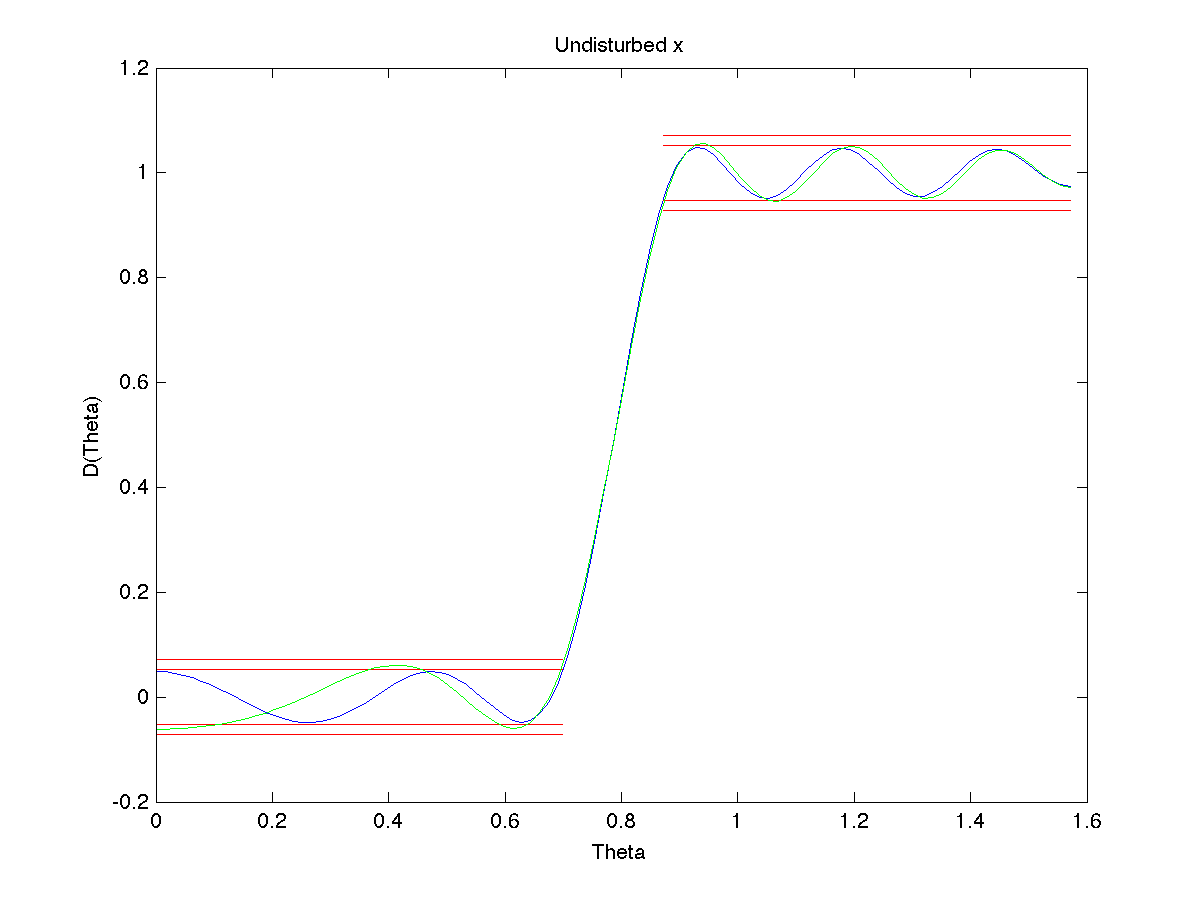
\includegraphics[width=\textwidth]{D-ModRobustCon.png}
  \end{subfigure}
  ~ 
 \begin{subfigure}[b]{0.32\textwidth}
  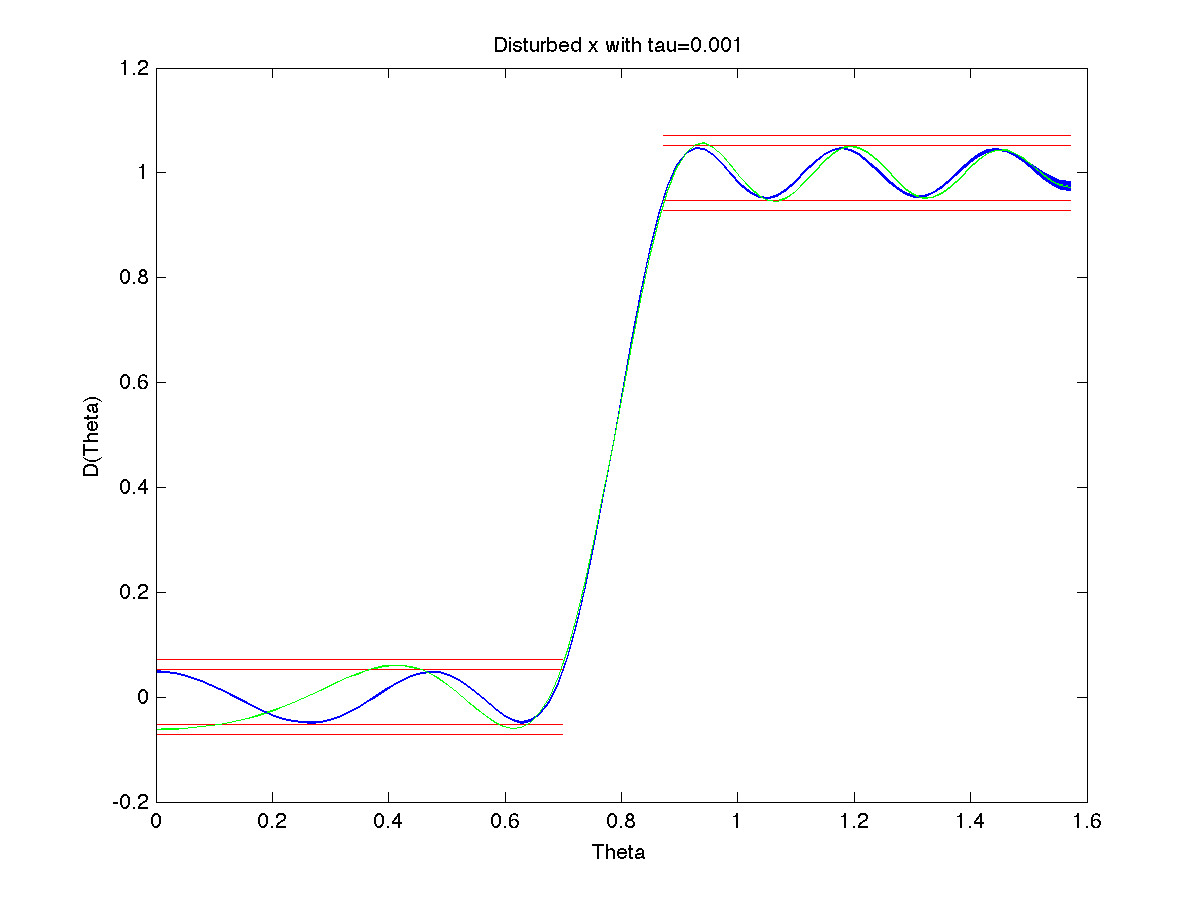
\includegraphics[width=\textwidth]{D-ModRobustCon-tau0001.png}
  \end{subfigure}
  \begin{subfigure}[b]{0.32\textwidth}
  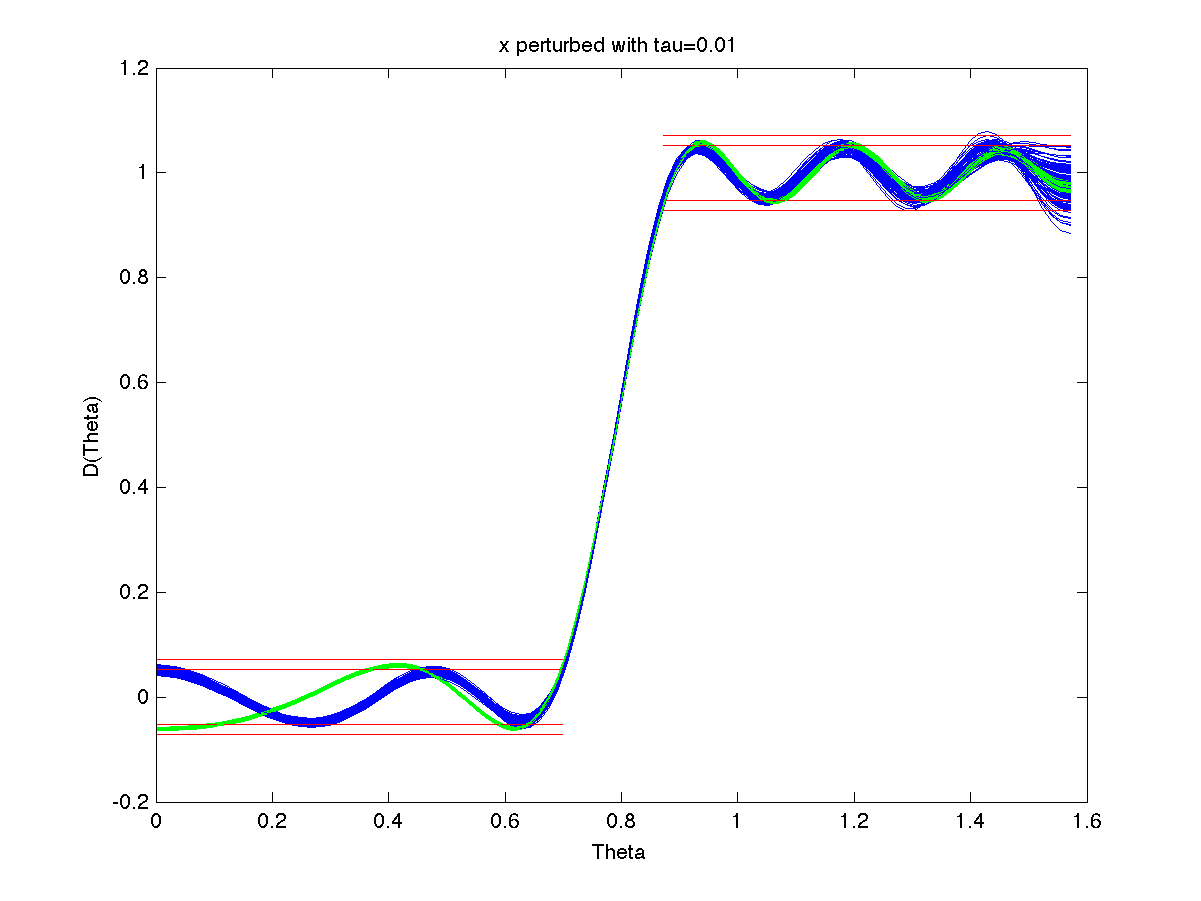
\includegraphics[width=\textwidth]{D-ModRobustCon-tau001.png}
  \end{subfigure}
\caption{Graphes de $D(\theta)$ pour des $x$ non-perturbés, avec une perturbation $\tau=0.001$ et avec une perturbation $\tau = 0.01$(en vert pour un modèle de $\tau=0.01$ en bleu pour $\tau=0.001$). Les deux derniers graphes sont donnés pour une centaine de réalisations des $\xi_i$.}
  \label{fig:D-ModCon}

  \end{figure}

\end{document}